\documentclass[latex/main.tex]{subfiles}

\begin{document}
\section{Results}

This section presents simulation results and timescale maps from resting fMRI (rfMRI). It compares the \nameref{sec:time-domain-linear-model} and \nameref{sec:autocorrelation-domain-nonlinear-model} methods in terms of timescale estimates, standard errors, t-statistics, and relative standard errors, highlighting differences in finite sample bias and variance. Three simulation settings are shown (see \nameref{sec:simulations}): AR1 \ref{fig:sim-ar1}, AR2 \ref{fig:sim-ar2}, and empirical \ref{fig:sim-hcp}. Additionally, brain timescale maps from the Human Connectome Project are included for an individual \ref{fig:map-hcp1} and group \ref{fig:map-hcp180}, showing spatial patterns and reliability metrics across brain regions.


\begin{figure}[!ht]
    \centering
    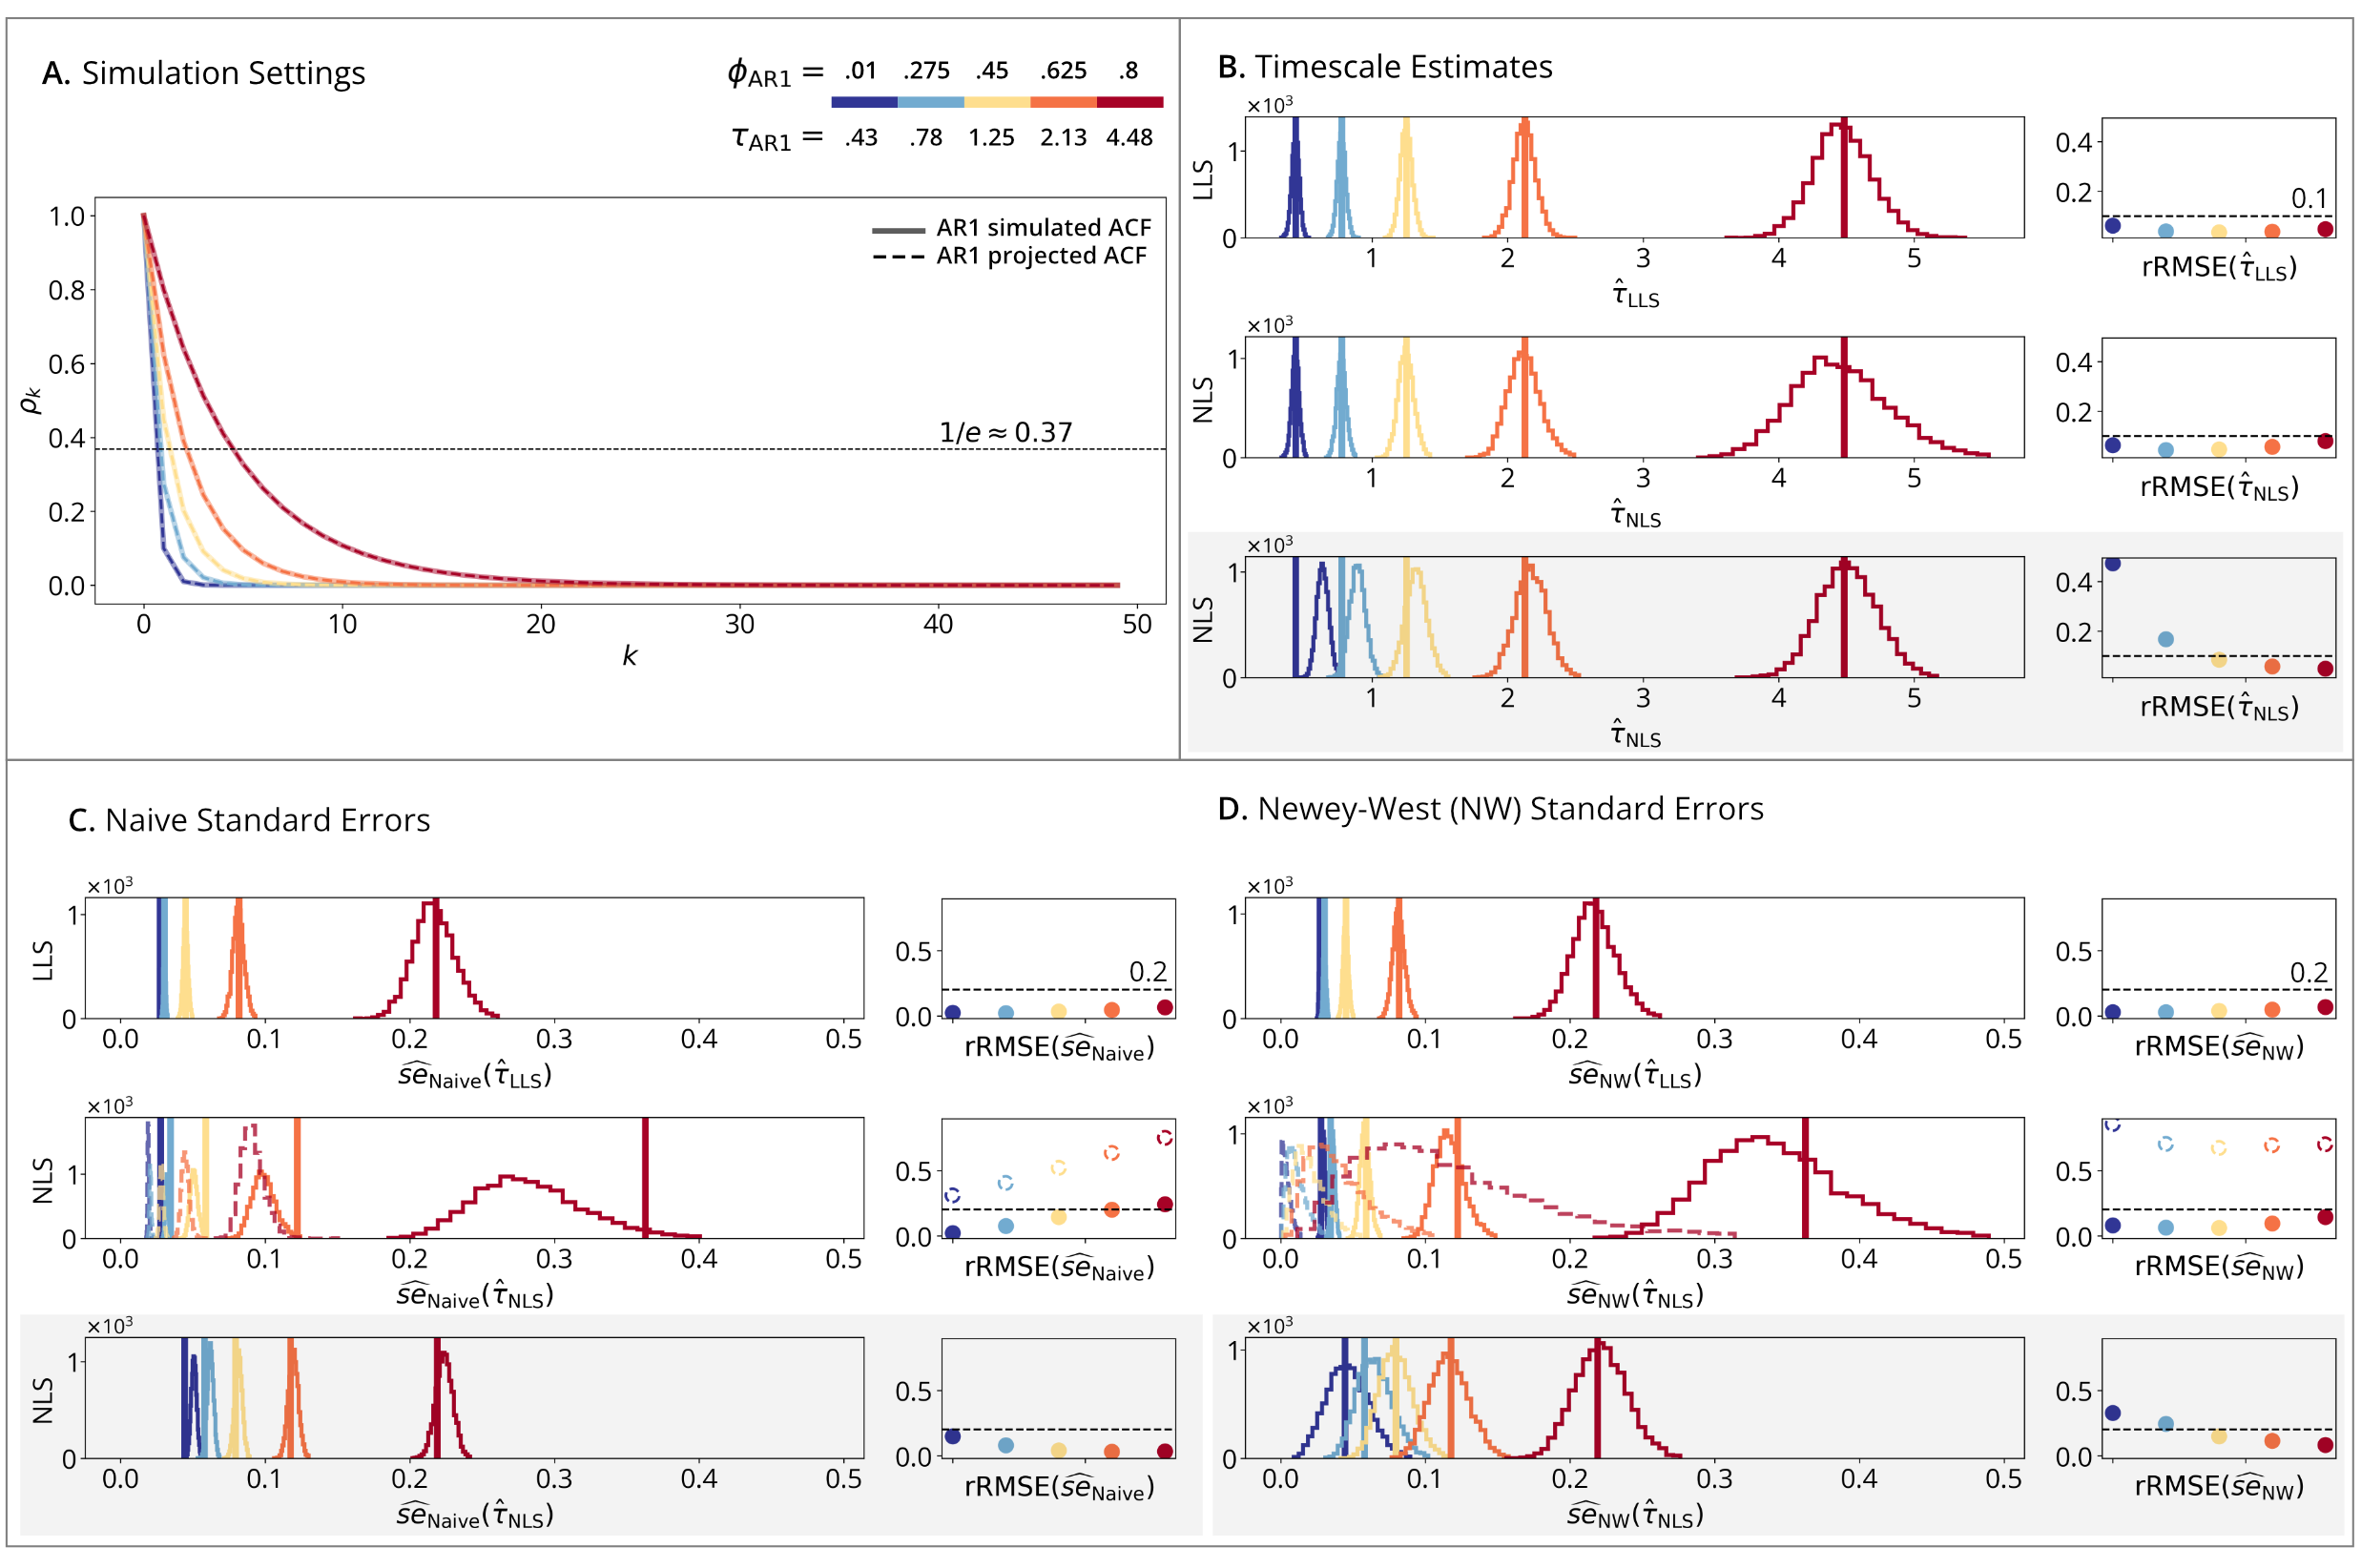
\includegraphics[width=1\textwidth]{figures/fig01-ar1.png} 
    \caption{\textbf{AR1 simulations.}}
    \subcaption*{
    (\textbf{A}) Simulation Settings. Five fixed settings are illustrated, where the solid line represents the simulated autocorrelation function (ACF), and the dashed line represents the AR1-projected ACF. Since both ACFs follow AR1, they overlap. Solid dots mark the timescale at which the AR1-projected ACF reaches $1/e \approx 0.37$.
    (\textbf{B}) Timescale Estimates. Vertical lines show the true timescale parameters, and histograms show the distribution of timescale estimates across $N=10,000$ independent replications. The top plot shows the results for the linear least squares estimator (LLS), and the bottom plot for the nonlinear least squares estimator (NLS).
    (\textbf{C}) Naive Standard Errors and (\textbf{D}) Newey-West Standard Errors. Vertical lines show the standard deviations of the sampling distributions from panel B, while histograms show the distribution of standard error estimates using the naive and Newey-West estimators, respectively.
    (\textbf{E}) T-Statistics and (\textbf{F}) Relative Standard Errors (RSEs). Vertical lines show true values and histograms show the distributions of the estimates. 
    }
    \label{fig:sim-ar1}
\end{figure}

\begin{figure}[!ht]
    \centering
    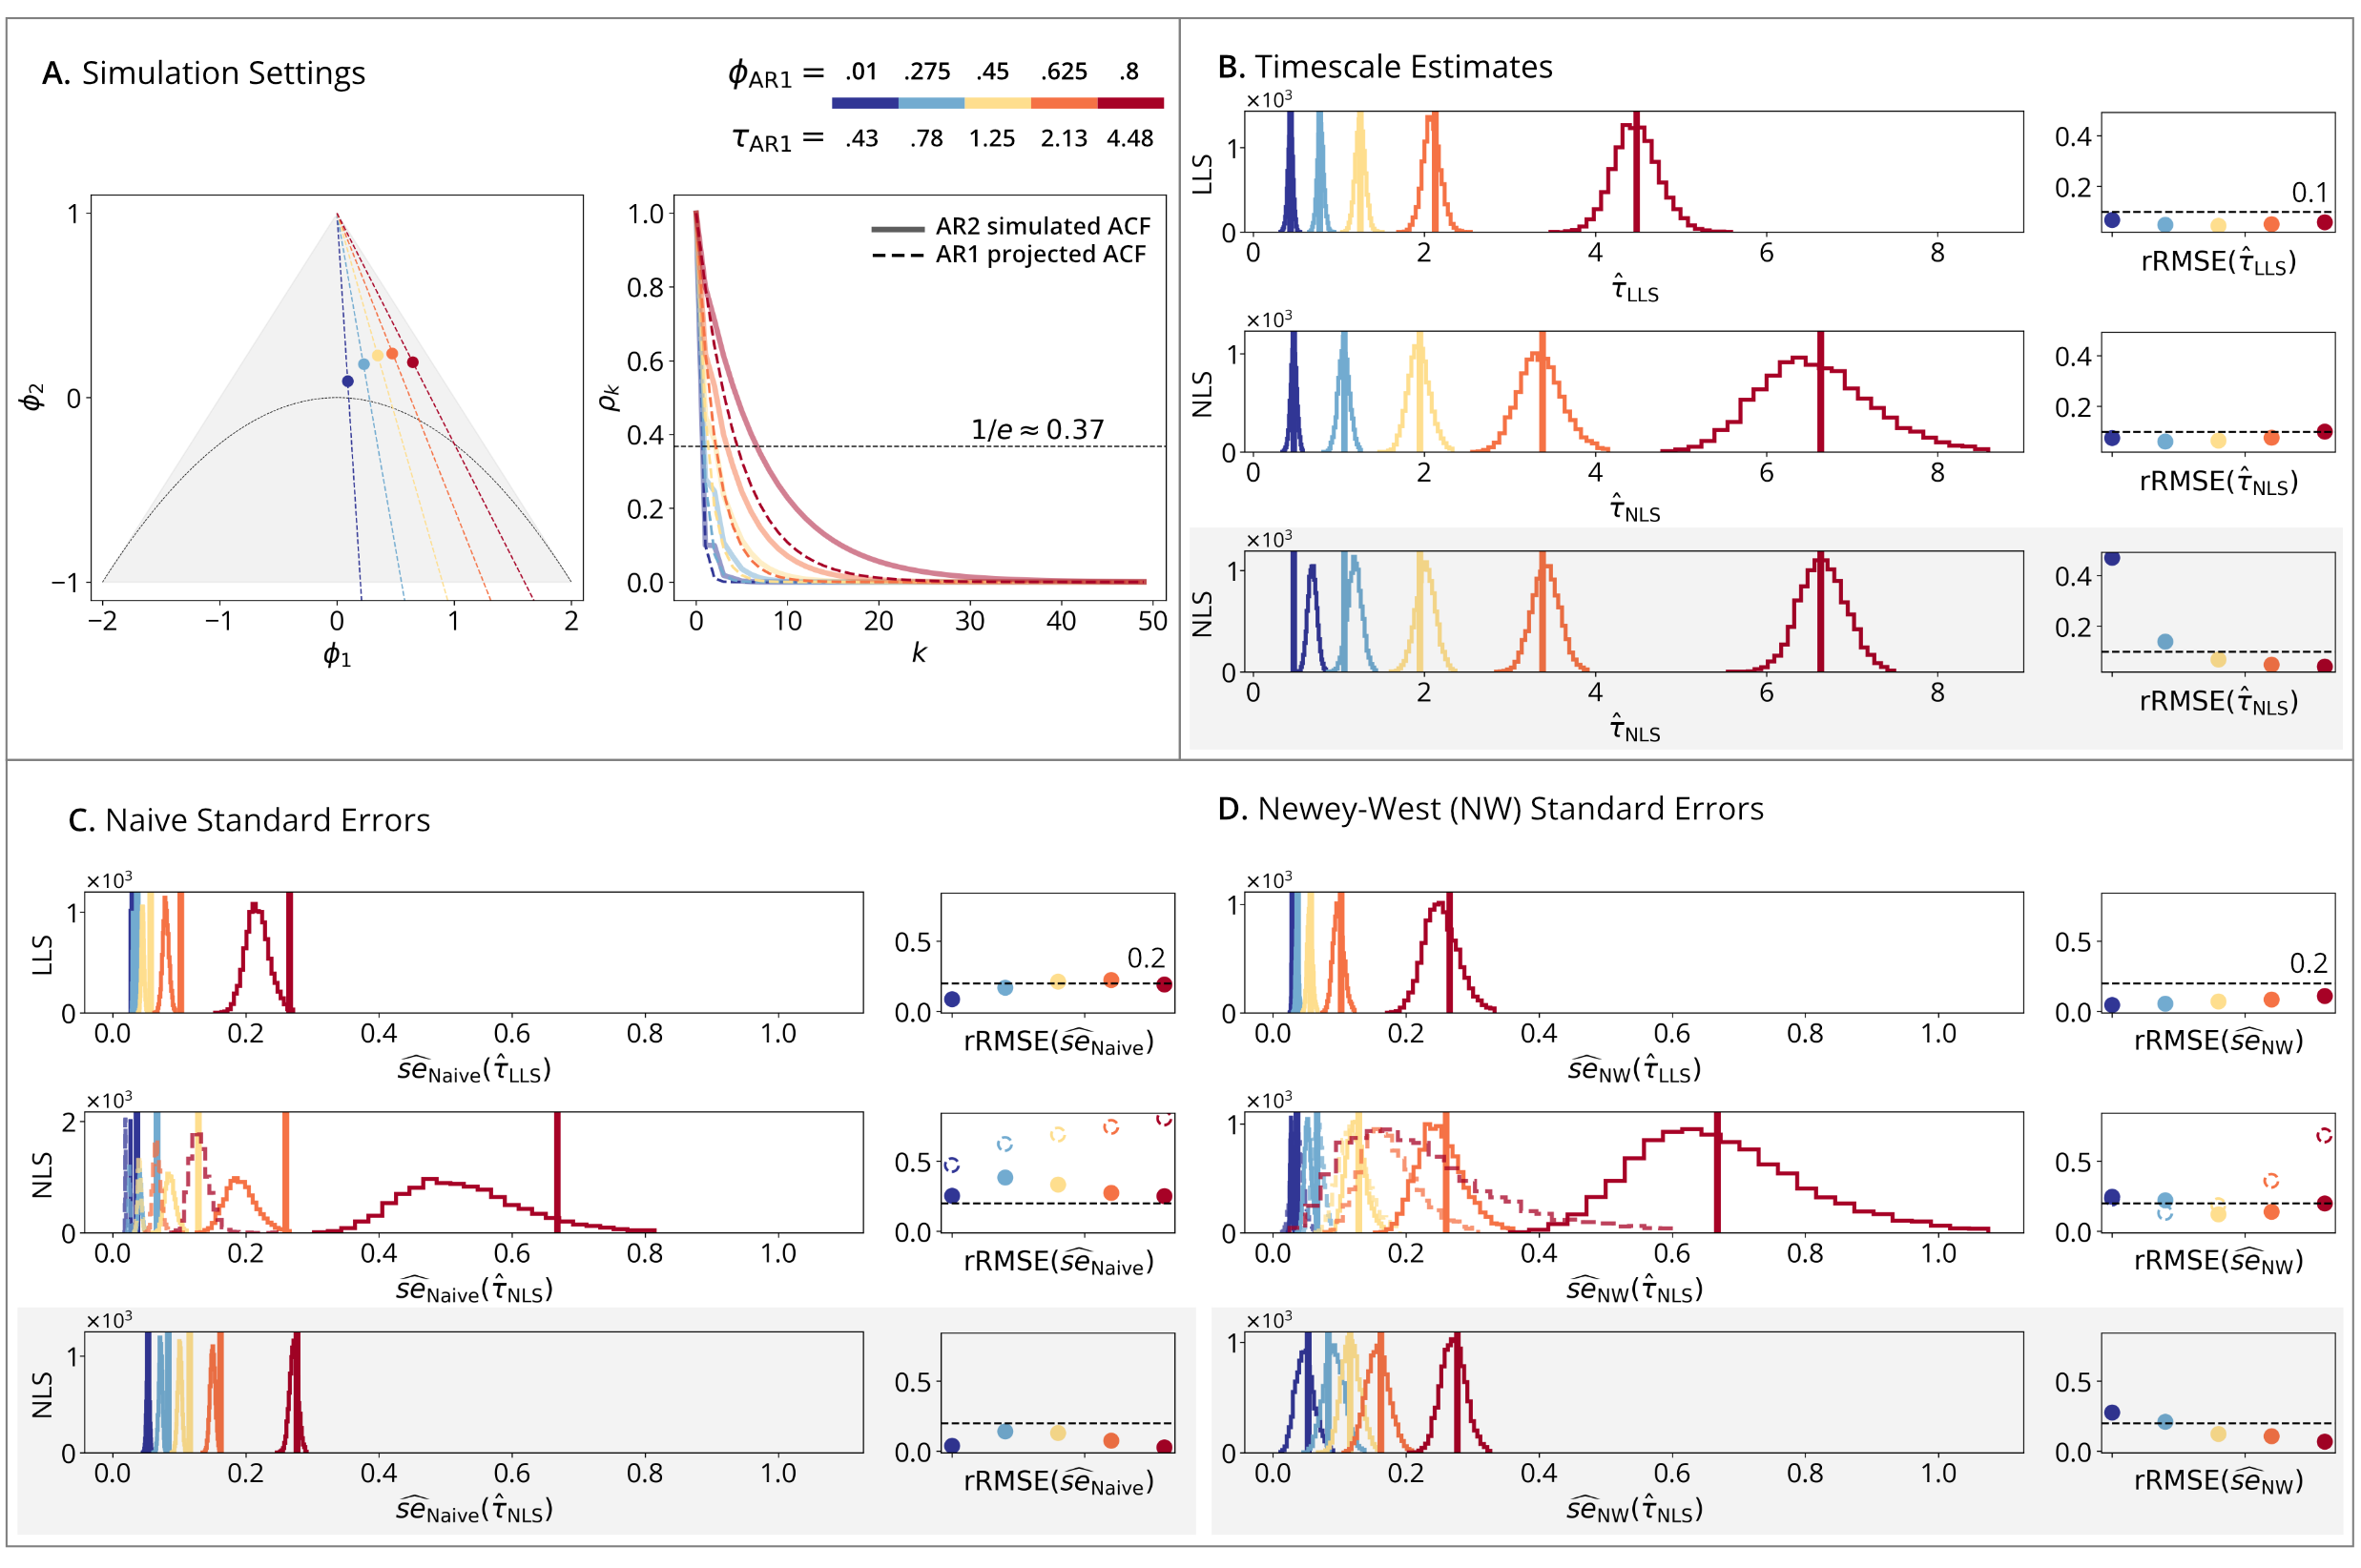
\includegraphics[width=1\textwidth]{figures/fig02-ar2.png} 
    \caption{\textbf{AR2 simulations.}}
    \subcaption*{
    (\textbf{A}) Simulation Settings. The AR2 stationary region (gray triangle) in the $(\phi_1, \phi_2)$ plane is defined by the conditions $\phi_2<1+\phi_1, \phi_2<1-\phi_1, \phi_2>-1$. Within this region, the theoretical boundary between periodic and aperiodic behavior is given by $\phi_2 = -\phi_1^2/4$. Five fixed $(\phi_1, \phi_2)$ pairs within the stationary and aperiodic region were used to simulate AR2 processes with AR1 projections (dashed lines) equivalent to Figure \ref{fig:sim-ar1}. In the autocorrelation domain, the solid lines represents the simulated autocorrelation function (ACF), and the dashed line represents the AR1-projected ACF. Since the simulated ACF is AR2 and the projected is AR1, the lines do not overlap. Solid dots mark the timescale at which the AR1-projected ACF reaches $1/e \approx 0.37$.
    (\textbf{B}) Timescale Estimates. Vertical lines show the true timescale parameters, and histograms show the distribution of timescale estimates across $N=10,000$ independent replications. The top plot shows the results for the linear least squares estimator (LLS), and the bottom plot for the nonlinear least squares estimator (NLS). The true values of the two estimators differ because of their respective definitions.
    (\textbf{C}) Naive Standard Errors and (\textbf{D}) Newey-West Standard Errors. Vertical lines show the standard deviations of the sampling distributions from panel B, while histograms show the distribution of standard error estimates using the naive and Newey-West estimators, respectively.
    (\textbf{E}) T-Statistics and (\textbf{F}) Relative Standard Errors (RSEs). Vertical lines show true values and histograms show the distributions of the estimates.
    }
    \label{fig:sim-ar2}
\end{figure}


\begin{figure}[!ht]
    \centering
    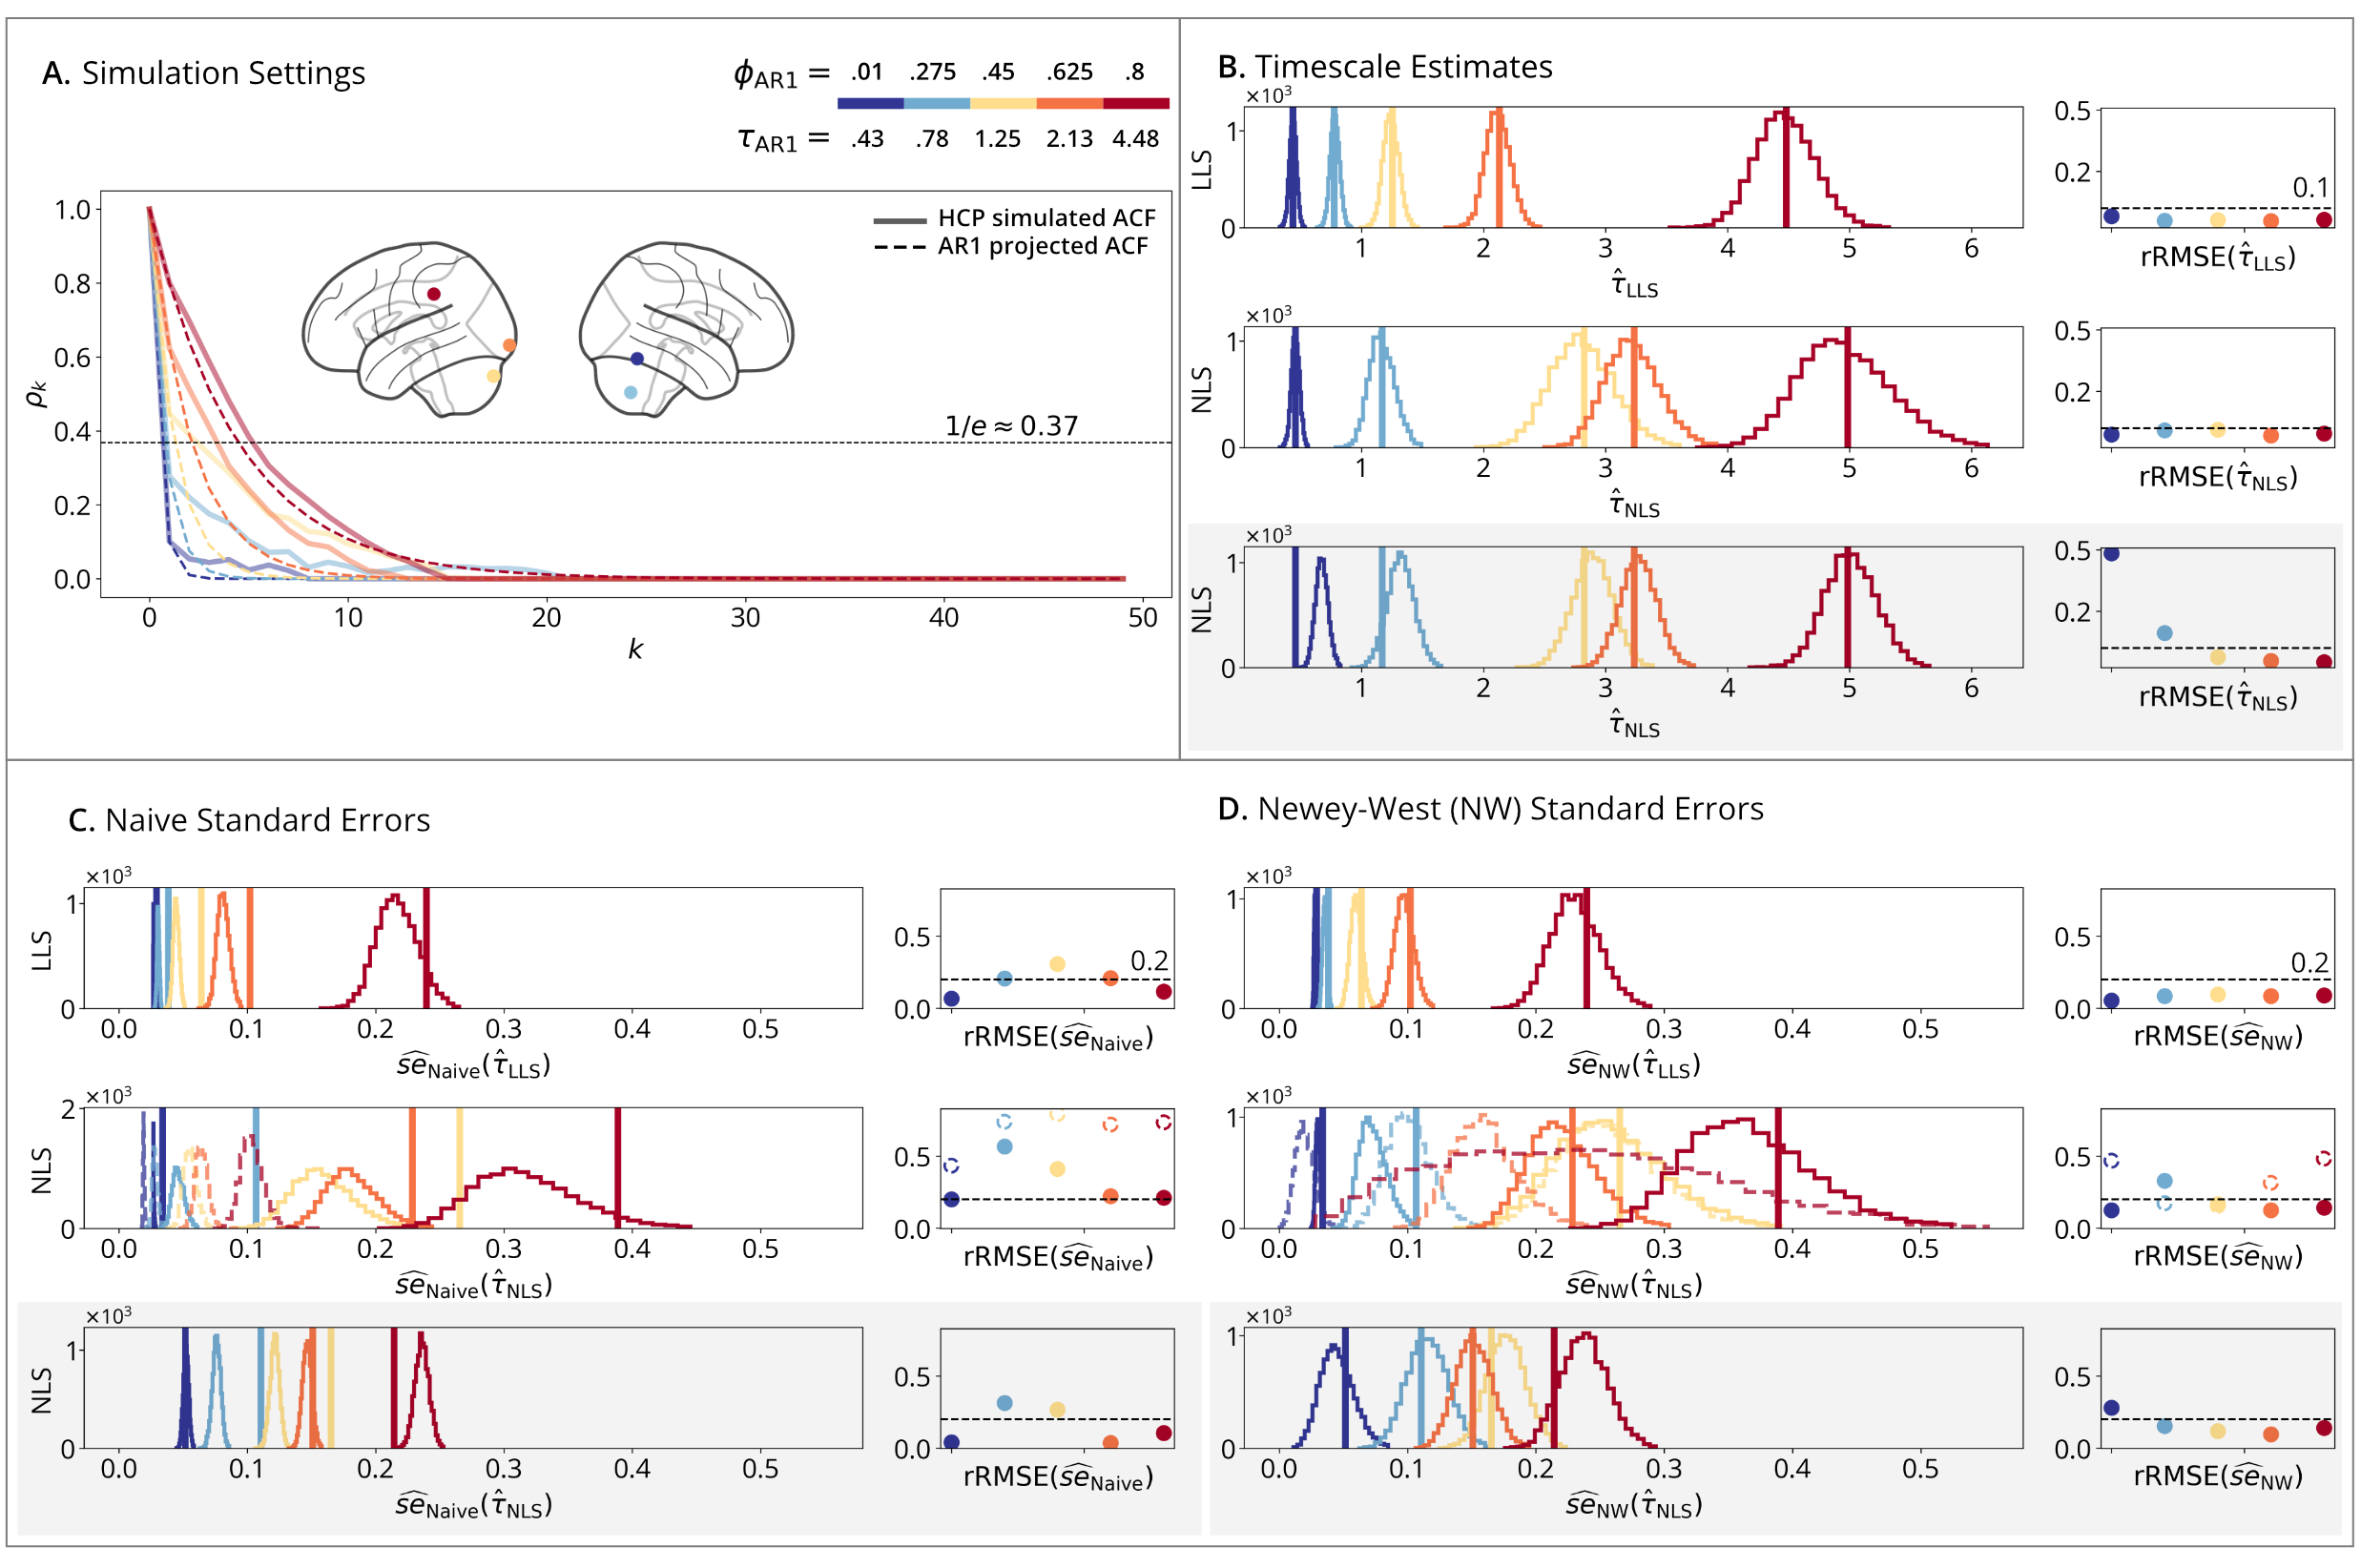
\includegraphics[width=1\textwidth]{figures/fig03-hcp.png} 
    \caption{\textbf{Realistic rfMRI simulations.}}
    \subcaption*{
    (\textbf{A}) Simulation Settings. Five fixed settings are illustrated, where the solid line represents the simulated autocorrelation function (ACF) of the specified brain region from subject $\#100610$ of the Human Connectome Project, and the dashed line represents the AR1-projected ACF. Since the simulated ACF depends on rfMRI data and the projected is AR1, the lines do not overlap. Solid dots mark the timescale at which the AR1-projected ACF reaches $1/e \approx 0.37$.
    (\textbf{B}) Timescale Estimates. Vertical lines show the true timescale parameters, and histograms show the distribution of timescale estimates across $N=10,000$ independent replications. The top plot shows the results for the linear least squares estimator (LLS), and the bottom plot for the nonlinear least squares estimator (NLS). The true values of the two estimators differ because of their respective definitions.
    (\textbf{C}) Naive Standard Errors and (\textbf{D}) Newey-West Standard Errors. Vertical lines show the standard deviations of the sampling distributions from panel B, while histograms show the distribution of standard error estimates, using the naive and Newey-West estimators, respectively.
    (\textbf{E}) T-Statistics and (\textbf{F}) Relative Standard Errors (RSEs). Vertical lines show true values and histograms show the distributions of the estimates.
    }
    \label{fig:sim-hcp}
\end{figure}

\subsection{\textit{Timescale Estimators in Autoregressive Simulations}}

AR1 simulation results (Figure \ref{fig:sim-ar1}) follow the setting where the data-generating process aligns with the fitted models, where each time series is generated from a first-order autoregressive process (fit by LLS) and each ACF by an exponential decay process (fit by NLS). The figure panels show how accurately the timescale estimators recover the true parameters and their standard errors as the timescale increases. \textbf{Panel B} shows that larger timescales lead to greater variability in the estimates, indicated by wider sampling distributions. Comparing the estimators, LLS remains unbiased across all timescales, while NLS exhibits upward bias at smaller timescales. \textbf{Panels C and D} compare the naive and Newey-West standard errors. Both estimators are unbiased, but standard errors increase as the timescales grow. The Newey-West estimator displays greater variability in standard error estimates compared to the naive estimator. This pattern holds for NLS as well, though the increase in variability is less pronounced, and the naive standard errors are overestimated for smaller timescales. \textbf{Panel E} examines t-statistics (signal-to-noise ratios). For LLS, the t-ratios fluctuate as timescales increase, while NLS shows a steady rise, indicating that larger timescales are easier to estimate. Across all timescales (except for the largest, $\tau_\text{AR1} = 4.48$), LLS outperforms NLS in terms of signal-to-noise ratios, and \textbf{Panel F} confirms that LLS also has lower RSEs. Overall, when both LLS and NLS are correctly specified they achieve nominal bias (i.e., they recover the true timescales and standard errors), though LLS is more reliable for small timescales.\\

AR2 simulation results (Figure \ref{fig:sim-ar2}) explore how timescale estimators perform when the data-generating model is AR2, introducing misspecification since the estimators fit AR1 projections. In this setting, the goal is to assess the impact of specification error on timescale estimation. \textbf{Panel A} illustrates the AR2 autocorrelation function (ACF) and its AR1 projection, emphasizing the mismatch between the true and fitted models. \textbf{Panel B} shows that the true timescale differs between the two estimators due to their respective definitions. Despite the misspecification, both timescale estimators remain (mostly) unbiased. However, the standard error estimates for both LLS and NLS are biased downward, particularly at larger timescales. The Newey-West estimator reduces this bias, improving the accuracy of standard error estimates for both models. \textbf{Panels E-F} show that, similar to the AR1 case, the LLS compared to the NLS estimator generally achieves larger t-statistics (indicating a higher signal-to-noise ratio) and lower RSEs. Additionally, larger timescales are easier to estimate, particularly for the LLS estimator. In summary, the Newey-West estimators can recover the true standard errors under model misspecification, larger timescales are generally easier to estimate, and the LLS estimator is more reliable for small timescales.

\subsection{\textit{Timescale Estimators in Realistic rfMRI Simulations}}

Realistic rfMRI simulation results (Figure \ref{fig:sim-hcp}) explore the performance of timescale estimators when simulating empirical processes derived from five distinct brain regions from a single subject. Like the AR2 results described above, this simulation method is designed to test estimator performance under model misspecification, as the data-generating process reflects realistic brain dynamics, while the fitted models project a simpler AR1 process. \textbf{Panel A} shows the empirical ACFs from these brain regions alongside their AR1 projections, highlighting the mismatch between the true underlying processes and the fitted models. \textbf{Panel B} presents the timescale estimates, where the LLS and NLS estimators yield different timescales due to their respective definitions. The naive standard error estimator for LLS consistently exhibits downward bias, while the NLS naive estimator shows bias that varies in direction depending on the timescale. For both methods, the Newey-West standard error estimates mitigate these biases, though they increase the variability of the estimates, particularly for NLS. \textbf{Panels E-F} display the t-statistics and RSEs, respectively, with LLS again demonstrating more stable and lower RSEs compared to NLS across most timescales. Larger timescales are consistently easier to estimate, and the Newey-West corrections effectively reduce bias, albeit at the cost of greater variability. These results are consistent with the AR2 simulations using a setting that is more realistic for estimating rfMRI timescale maps.

\begin{figure}[!ht]
    \centering
    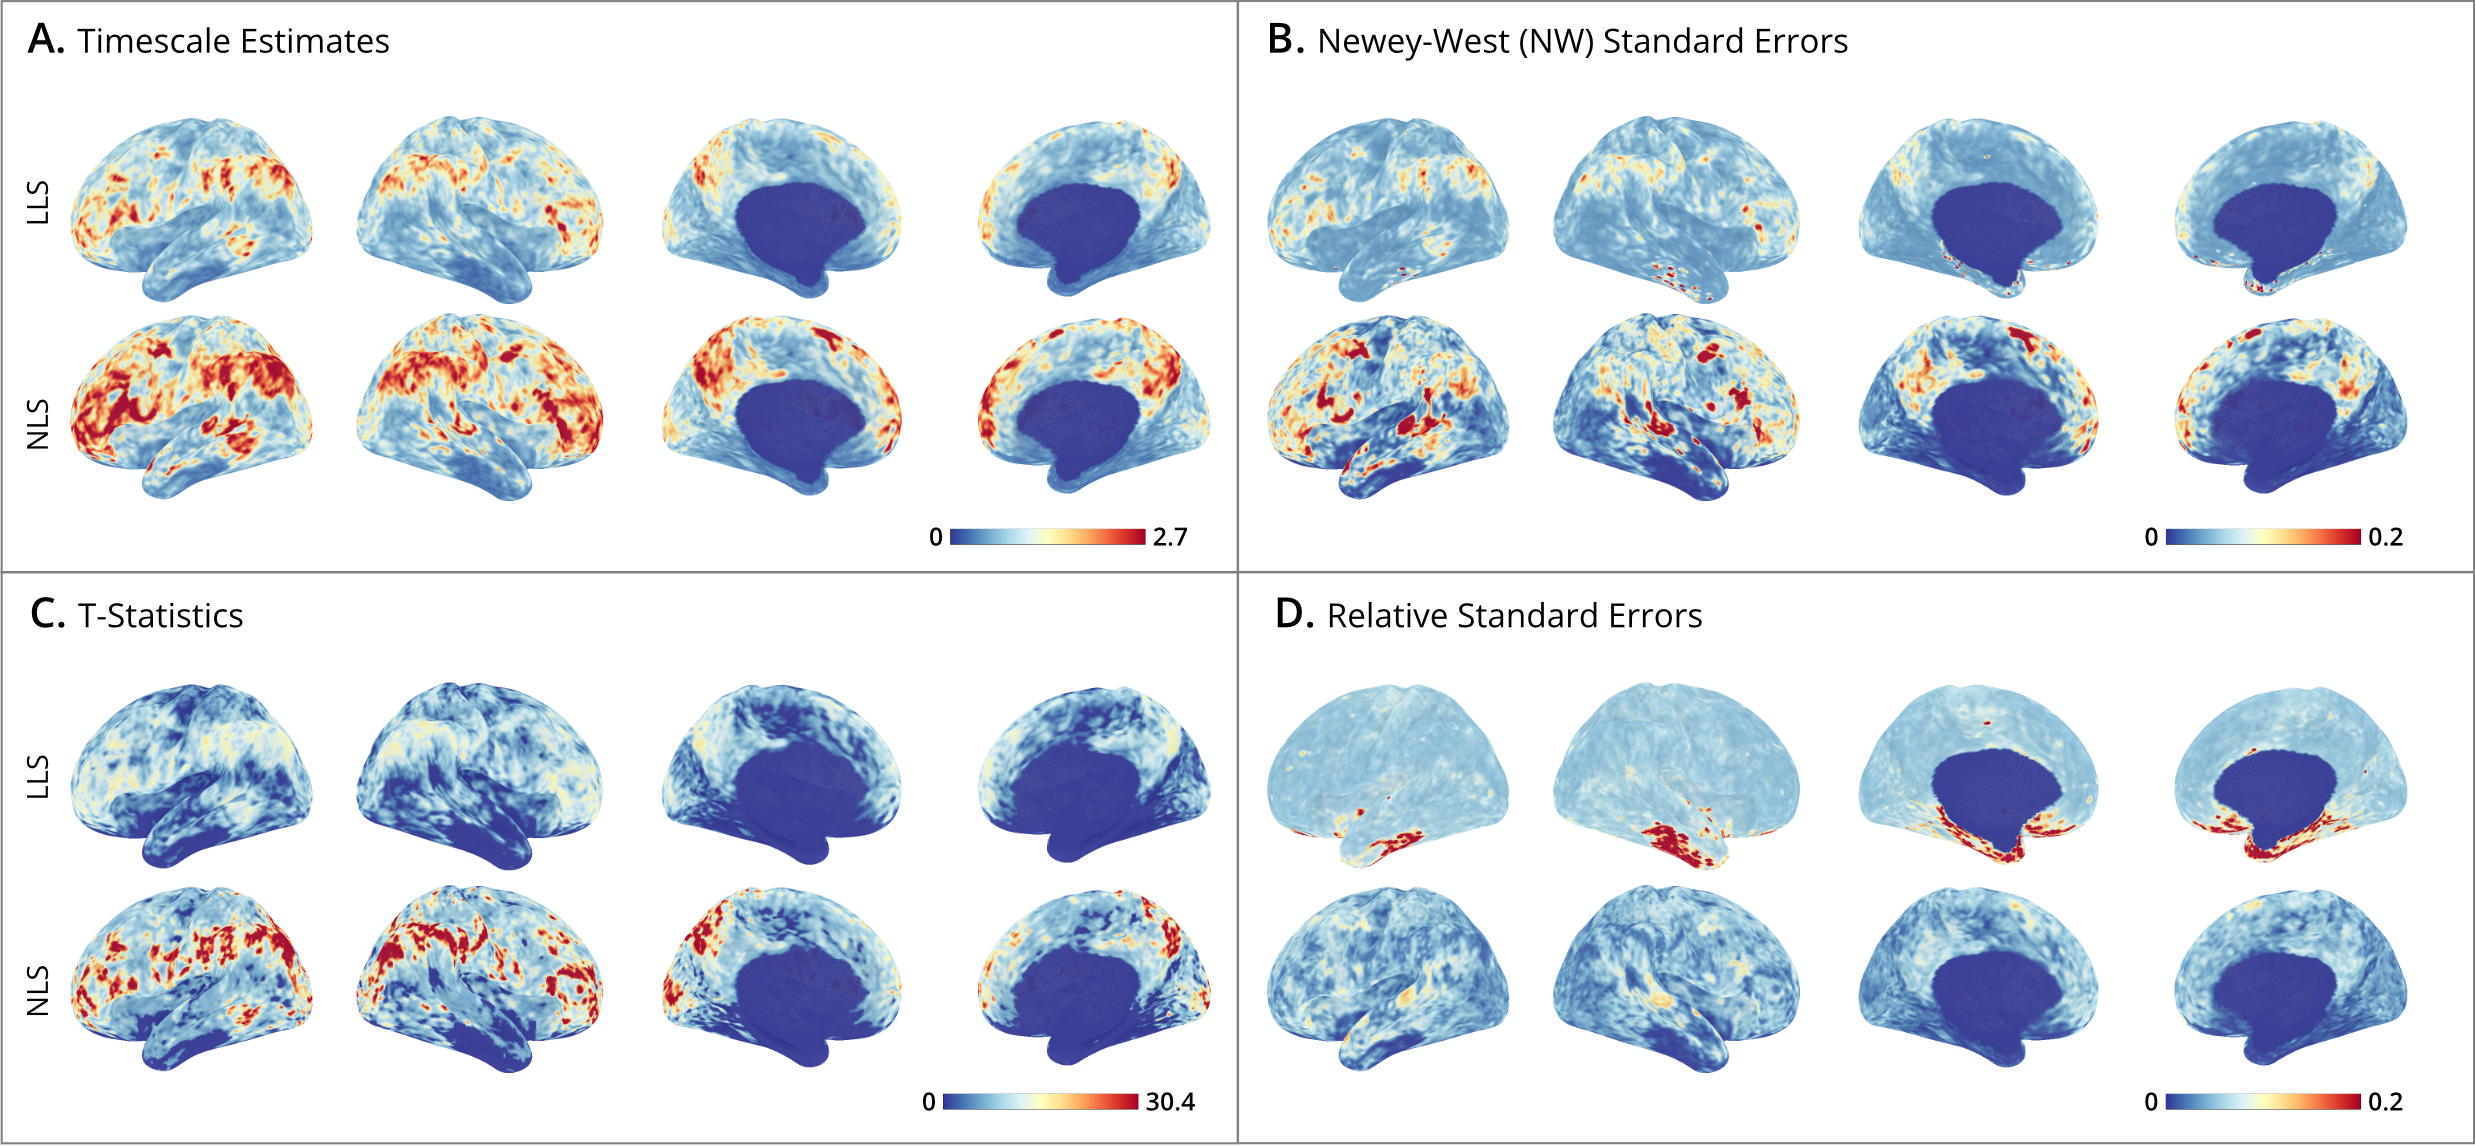
\includegraphics[width=1\textwidth]{figures/fig04-hcp1.png} 
    \caption{\textbf{Human Connectome Project subject-level timescale maps.}}
    \subcaption*{
    (\textbf{A-D}) panels display cortical gray-matter maps from subject $\# 100610$ of the Human Connectome Project. Displays include lateral-left, lateral-right, medial-left, and medial-right views (excluding the medial wall). The upper bounds on the colorbars are set for each panel at the $99^\text{th}$ percentile of the cortical map values. For each panel, the top row shows the results of linear least squares estimator (LLS), and the bottom row shows the results of the nonlinear least squares estimator (NLS). 
    \textbf{A} Timescale Estimates. Maps display the timescales (e-folding time in seconds) across brain regions. 
    \textbf{B} Newey-West Standard Errors. Maps display the spatial distribution of robust standard error estimates, with smaller values indicating greater precision in the timescale estimates. 
    \textbf{C} T-Statistics. Maps display unthresholded and uncorrected t-ratios, testing whether timescales at each grayordinate exceed a half second. 
    \textbf{D} Relative Standard Errors (RSEs). Values show the relative reliability of timescale estimates across brain regions. Low RSE (near zero) indicates high precision with small uncertainty, while higher RSE reflects lower reliability of the estimates.
    }
    \label{fig:map-hcp1}
\end{figure}

\begin{figure}[!ht]
    \centering
    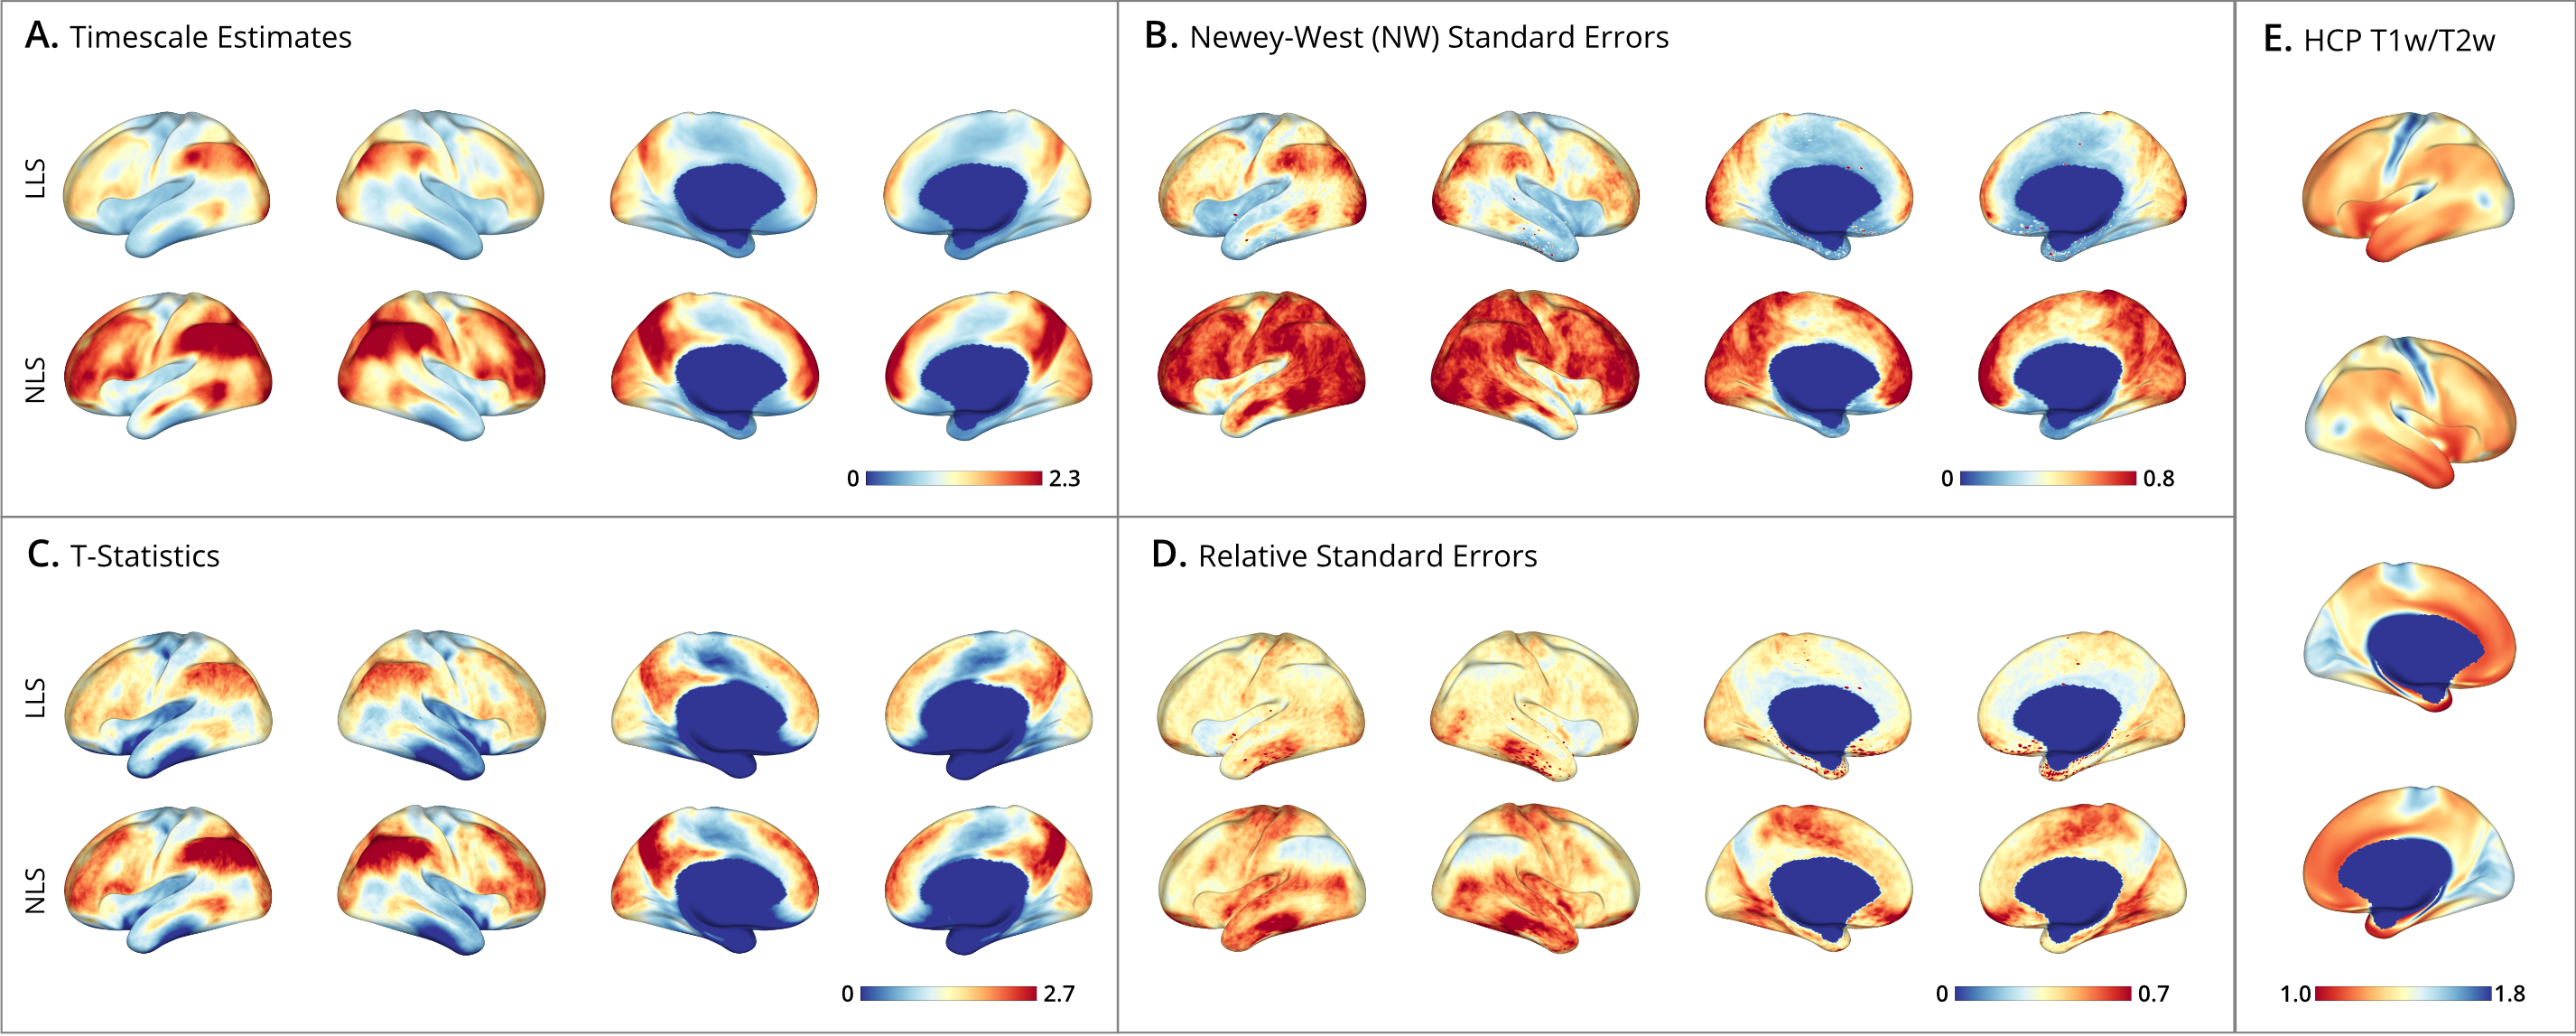
\includegraphics[width=1\textwidth]{figures/fig05-hcp180.png} 
    \caption{\textbf{Human Connectome Project group-level timescale maps.}}
    \subcaption*{
    (\textbf{A-D}) panels display cortical gray-matter maps from the group of $N=180$ subjects in the Human Connectome Project dataset. Displays include lateral-left, lateral-right, medial-left, and medial-right views (excluding the medial wall). The upper bounds on the colorbars are set for each panel at the $99^\text{th}$ percentile of the cortical map values. The top row in each panel shows results from the linear least squares estimator (LLS), and the bottom row shows results from the nonlinear least squares estimator (NLS). 
    \textbf{A} Timescale Estimates. Maps display the group-level timescales (e-folding time in seconds) across brain regions, averaged over subjects.
    \textbf{B} Newey-West Standard Errors. Group-level maps show the spatial distribution of standard error estimates, account for within-individual variability and between-individual variability. Smaller values indicate greater precision in the timescale estimates within and between subjects.
    \textbf{C} T-Statistics. Maps display unthresholded and uncorrected t-ratios, testing whether timescale at each surface coordinate exceed a half second.
    \textbf{D} Relative Standard Errors (RSEs). Maps show the relative reliability of timescale estimates across brain regions and subjects. Low RSE indicates high precision with small uncertainty, while high RSE suggests lower reliability of the estimates.
    \textbf{E} The T1w/T2w ratio from the Human Connectome Project maps cortical mylination, included here as a visual comparator to the spatial organization of timescales. This ratio is a useful proxy for mapping the sensory-associative axis of the brain, where sensory areas (e.g. primary visual and motor cortices; red) need fast signal transmission and high myeline levels, while associative regions (e.g. prefrontal cortex; blue) are less myelinated.
    }
    \label{fig:map-hcp180}
\end{figure}


\subsection{\textit{Estimation of rfMRI Timescale Maps}}
Subject-level timescale maps were derived from the Human Connectome Project dataset by independently fitting both LLS and NLS estimators to each cortical surface coordinate, using a mass-univariate approach to produce subject-level maps of timescale estimates and their associated standard errors. This method allows for spatially resolved estimates across the brain's cortical surface, enabling a detailed comparison of the two estimated timescale maps. \textbf{Panel A} presents the spatial distribution of timescale estimates, revealing that, consistent with the simulation results, NLS estimates tend to yield larger timescales than LLS. \textbf{Panel B} shows the corresponding maps of standard errors, which appear spatially correlated with the timescale estimates, consistent with the simulation finding that larger timescales are associated with greater sampling variability. \textbf{Panel C} depicts the relative ratio of timescale estimates to their standard errors (i.e., t-statistics), testing whether the timescales significantly exceed a half second ($H_0: \tau \leq 0.5$). Despite the larger standard errors for higher timescales, these regions exhibit higher t-statistics, particularly for the NLS estimator, where t-statistics extend further into the tail of the distribution, indicating stronger evidence against the null hypothesis. This result is in line with simulations, which demonstrated that NLS provides higher signal-to-noise ratios for very large timescales compared to LLS. \textbf{Panel D} shows low RSEs across much of the brain indicating high estimation reliability. Overall, the LLS and NLS methods show comparable spatial organization of timescales across the cortical surface, but they diverge at the extremes—NLS tends to estimate much larger timescales, while LLS is more reliable for very small timescales, consistent with their differing behavior in boundary cases observed in the simulations.\\

Group-level timescale maps were generated by combining individual estimates to account for both within-individual and between-individual variability, providing an aggregate view of timescale distributions across subjects. \textbf{Panel A} shows that the average timescale maps for both LLS and NLS estimators are smoother than the individual maps, displaying a well-organized spatial pattern across the cortex, with NLS estimates generally being larger than LLS. \textbf{Panel B} presents the standard error maps, which combine variances from within-subject Newey-West estimates and between-subject timescale estimates. As expected, the standard errors are larger for NLS than for LLS. \textbf{Panel C} depicts t-statistics testing whether timescales exceed a half second, showing that while both methods yield comparable results, NLS produces more extreme t-statistics. \textbf{Panel D} plots relative standard errors (RSEs), illustrating the general trend that regions with larger timescales are easier to estimate, while areas with smaller timescales exhibit greater uncertainty. Overall, these group-level maps highlight consistent spatial organization of timescales maps of the cortical surface. \textbf{Panel E} this organizing pattern has been compared in previous studies to the myelination gradient (T1w/T2w ratio), which aligns with the sensory-associative axis of brain function. At a very coarse approximation, this map appears weakly correlated with the timescale maps, where timescales increase from sensory to associative regions.
\end{document}